
\twocolumn[{%
\begin{center}
  {\LARGE \textbf{\textsf{Top Quark Seminar 9}}} \\
  \vspace{1em}
  {\Large \textbf{\textsf{Igor Babuschkin}}} \\
  \vspace{1em}
  {\large \textbf{\textsf{10th February 2015}}}
  \section*{Summary of \enquote{Top-tagging: A Method for Identifying Boosted Hadronic Tops}}
\end{center}
}]

\noindent
The paper\cite{kaplan} presents a novel technique for identifying top quarks in events where the top quark is highly boosted.

At the LHC most top quarks are created close to the $2m_t$ energy threshold.
If these slightly boosted top quarks decay hadronically, the $b$ jet is usually well separated from the other jets originating from light quarks.
The jets can be identified separately and then combined to form the top quark.

But if the top quark is highly boosted, the jets will overlap with high probability, which makes $b$-tagging difficult.
Highly boosted top quarks are an interesting testing ground for theories that introduce heavy particles that decay into top quarks, like most theories addressing the hierarchy problem.
As leptonic $t\overline{t}$ decays suffer from sizable dilepton backgrounds and $b$-tagging is difficult at high $p_T$, it would be useful to look at all-hadronic channels regardless of $b$-tags.

Top tagging, the approach presented by the authors, aims to identify top-quarks in precisely these types of events.
A previous technique\cite{brooijmans} manages to identify top quarks with an efficiency of \SI{45}{\percent} while rejecting \SI{95}{\percent} of the background.
This approach does not succeed in separating top quark events from the large dijet background.

Top tagging is based on analysing jet substructure:
After a standard clustering step, the resulting cluster is decomposed into two subclusters, each of which can be further decomposed if its fraction of the original cluster's $p_T$ is sufficiently high.
If a termination condition is met ($p_T$ fractions too small, clusters too close in the $η$-$φ$ plain, only one calorimeter cell left), the cluster is considered irreducible.
Clusters with 3 or 4 subclusters are kept and certain kinematic cuts are applied: the total invariant mass should be close to $m_t$, two subjets should reconstruct $m_W$ and the $W$ helicity angle should be consistent with a top quark decay.

To demonstrate the performance of their algorithm, the authors have prepared Monte Carlo samples of $t\overline{t}$ and dijet events and have applied their top-tagging algorithm.

\begin{figure}
  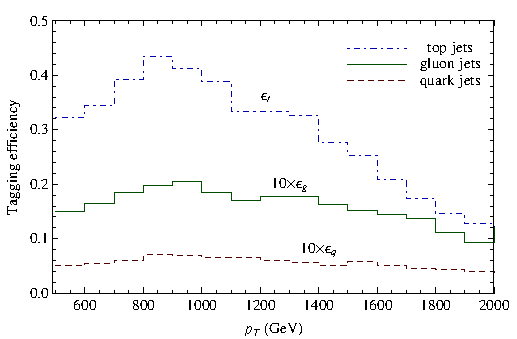
\includegraphics[width=0.5\textwidth]{figures/top-tagging-cropped.pdf}
  \caption{Efficiencies for correctly tagging a top quark $\varepsilon_t$, or for mistagging a quark or gluon ($\varepsilon_q$ and $\varepsilon_g$) using the top-tagging algorithm.\cite{kaplan}}
  \label{efficiencies}
\end{figure}

The resulting tagging (for the signal) and mistagging (for the background) efficiencies are displayed in figure \ref{efficiencies}.
The drop in tagging efficiency for the top quark at high $p_T$ results from the fact that the resolution of the calorimeter does not suffice to distinguish the individual subjets clearly.
The background rejection is on the order of one percent, which is a clear improvement compared to the previously mentioned alternative algorithm.

The authors also study how the invariant mass distributions of $t\overline{t}$ events and background events is affected by the top tagging algorithm.
They find that the dijet background is reduced greatly, to the level of the standard model $t\overline{t}$ prediction.
They conclude that this would make possible the detection of several kinds of new physics that produce a peak in the invariant mass of the $t\overline{t}$ distribution.

